\documentclass[11pt,a4paper]{article}

% ==========================================
% PACKAGES & FORMATTING
% ==========================================
\usepackage[margin=1in]{geometry}
\usepackage{graphicx}
\usepackage{amsmath, amssymb}
\usepackage{booktabs}
\usepackage{caption}
\usepackage{subcaption}
\usepackage{float}
\usepackage{hyperref}

% Differentiate figures/tables from main text
\renewcommand{\thefigure}{S\arabic{figure}}
\renewcommand{\thetable}{S\arabic{table}}
\renewcommand{\theequation}{S\arabic{equation}}
\renewcommand{\thesection}{S\arabic{section}}

\title{\Large \textbf{Supplementary Material for:\\Networks Decide for Us: Emergence of Adoption in Homophily-Imputed Social Topologies}}
\author{Aníbal Olivera Morales, Jorge Fábrega Lacoa, Thomas W. Valente}
\date{March 27, 2026}

\begin{document}

\maketitle
\tableofcontents
\vspace{1cm}

% ==========================================
% SECTION S1
% ==========================================
\section{Survey Items and Propensity Distributions}

To assign behavioral propensities (Minimum Utility Requirements, $q_i$) to the agents in our imputed topologies, we utilized specific batteries of items from the American Trends Panel (ATP). 

\subsection{Openness to Innovation Score (ATP 2014)}
The openness to innovation score was constructed using binary responses to the following items:
\begin{enumerate}
    \item Usually try new products before others do. (\textit{Pro-innovation})
    \item Prefer my tried and trusted brands. (\textit{Anti-innovation})
    \item Like being able to tell others about new brands and products I have tried. (\textit{Pro-innovation})
    \item Like the variety of trying new products. (\textit{Pro-innovation})
    \item Feel more comfortable using familiar brands and products. (\textit{Anti-innovation})
    \item Wait until I hear about others' experiences before I try new products. (\textit{Anti-innovation})
\end{enumerate}

\subsection{Collective Action Propensity Score (ATP 2016)}
For collective action simulations, the propensity score was generated from responses regarding political and social participation. Respondents indicated whether they had engaged in actions (e.g., in the past year, distant past, might do it, or would never do it):
\begin{enumerate}
    \item Signed a petition.
    \item Boycotted, or deliberately bought, certain products.
    \item Took part in a demonstration.
    \item Attended a political meeting or rally.
    \item Contacted a politician or a civil servant to express views.
    \item Donated money or raised funds for a social/political activity.
    \item Contacted or appeared in the media to express views.
    \item Joined an Internet political forum or discussion group.
\end{enumerate}

\subsection{Collective-Action Propensity: Construct Internal Reliability}
To ensure the empirical plausibility of the ATP mapping, we derive a unidimensional Minimum Utility Requirement (MUR) score. 
[PLACEHOLDER: Add Cronbach's alpha reliability test to verify multi-item unidimensionality for the collective-action propensity construct]. 

\subsection{Empirical Distribution of the Intrinsic Utility Level (IUL) / MUR}
The following distribution histograms (Figure \ref{fig:mur_dist}) reflect the normalized scores extracted from the ATP and GSS micro-data. We leverage the GSS structure for Figure 1 in the main manuscript because its survey distribution allows for a more granular, finely binned \textit{collective-action propensity score}. This expanded level-count avoids artifactual stepping and renders smooth analytical heatmaps capable of correctly tracing criticality variance signatures across contiguous thresholds.

\begin{figure}[H]
    \centering
    \begin{subfigure}[b]{0.45\textwidth}
        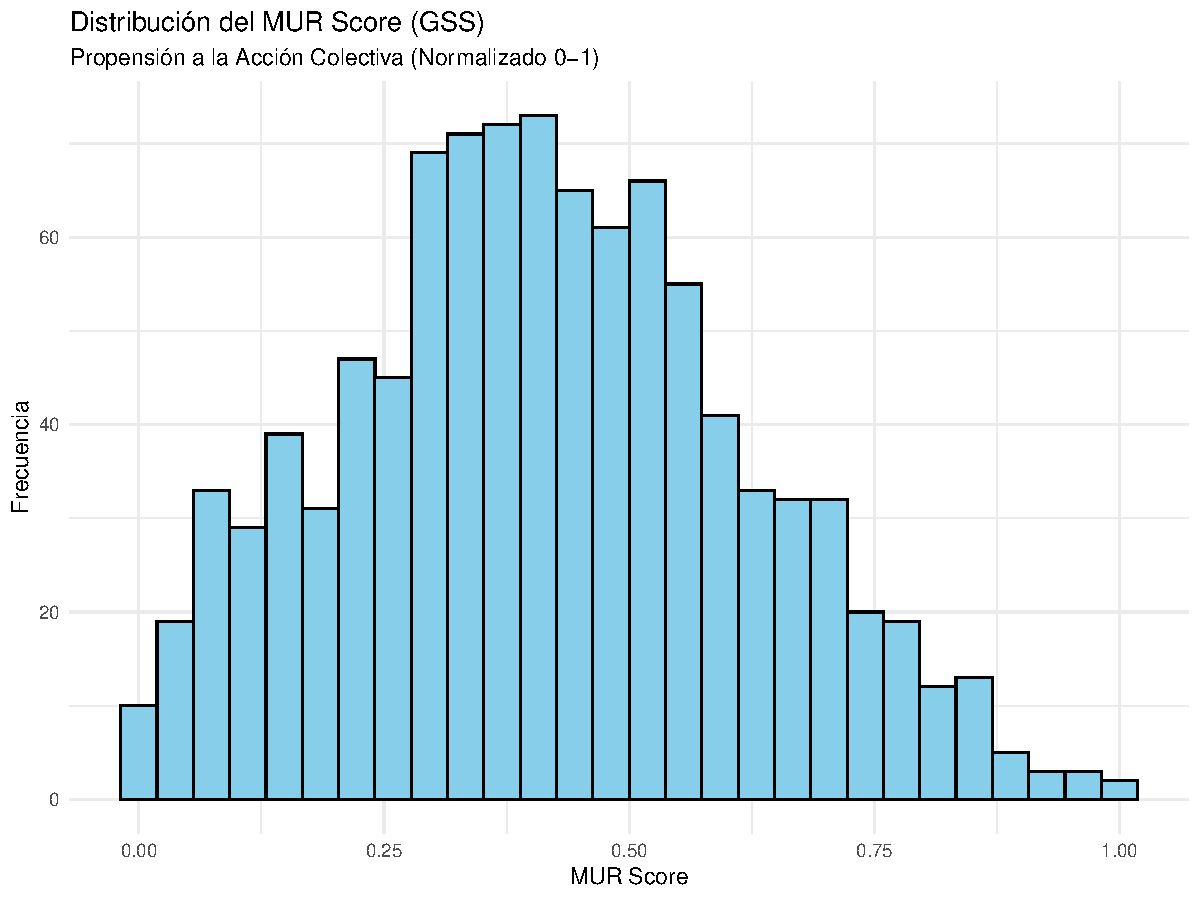
\includegraphics[width=\textwidth]{../../plots/03_GSS_MUR_calculation/GSS_mur_score_distribution.pdf}
        \caption{MUR Profile (GSS 2004).}
    \end{subfigure}
    \hfill
    \begin{subfigure}[b]{0.45\textwidth}
        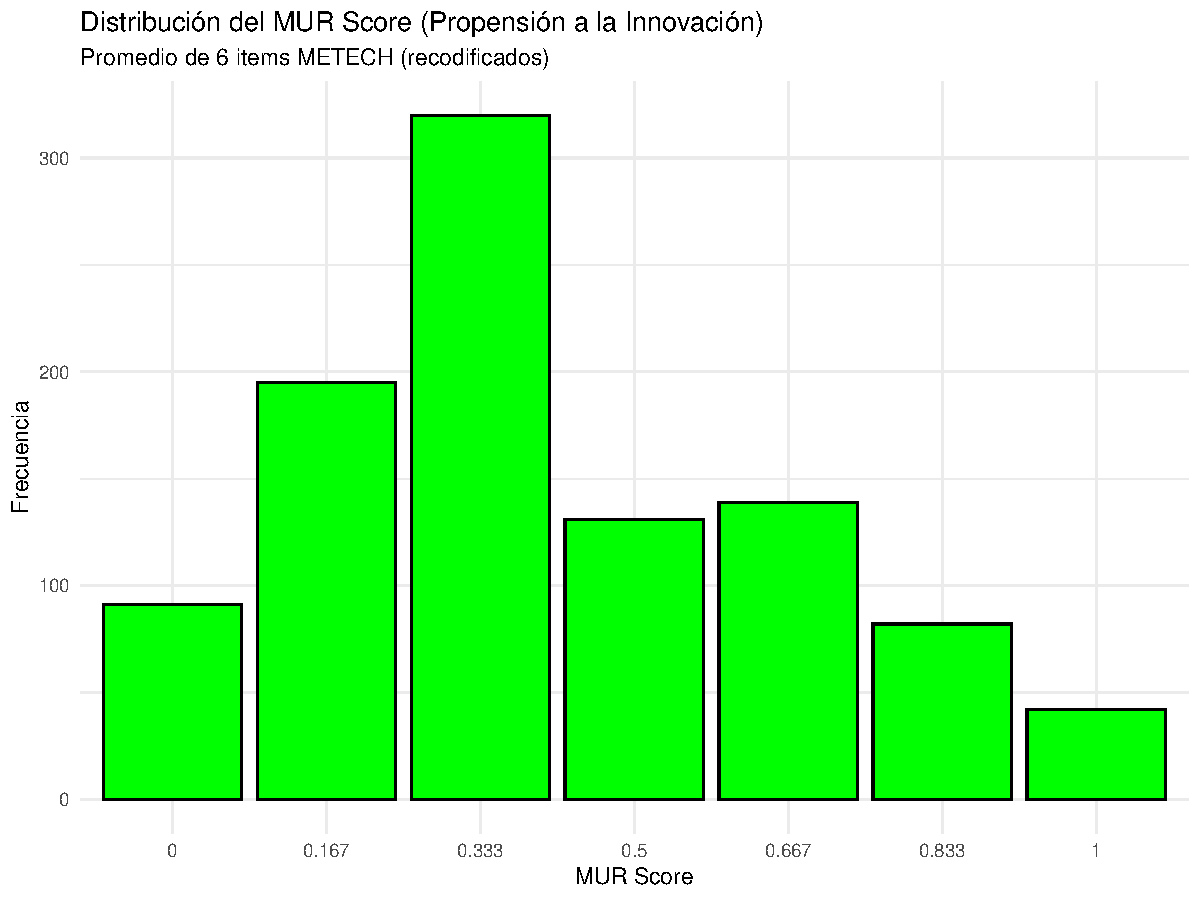
\includegraphics[width=\textwidth]{../../plots/03_ATP_MUR_calculation/ATP_mur_score_distribution.pdf}
        \caption{MUR Profile (ATP 2014/2016).}
    \end{subfigure}
    \caption{Distribution of Minimum Utility Requirements ($q_i$). Lower MUR implies higher propensity towards innovation.}
    \label{fig:mur_dist}
\end{figure}

\subsection{Criticality Heatmaps in Degree-Preserving Randomized Networks}
For direct comparison with the main structural signatures found across Plausible domains in the main text, Figure \ref{fig:criticality_er} documents the equivalent heatmaps corresponding to Degree-Preserving Randomized networks. This baseline identically preserves total node degree and density, but destroys local multidimensional homophily and structural clustering. 

\begin{figure*}[h]
    \centering
    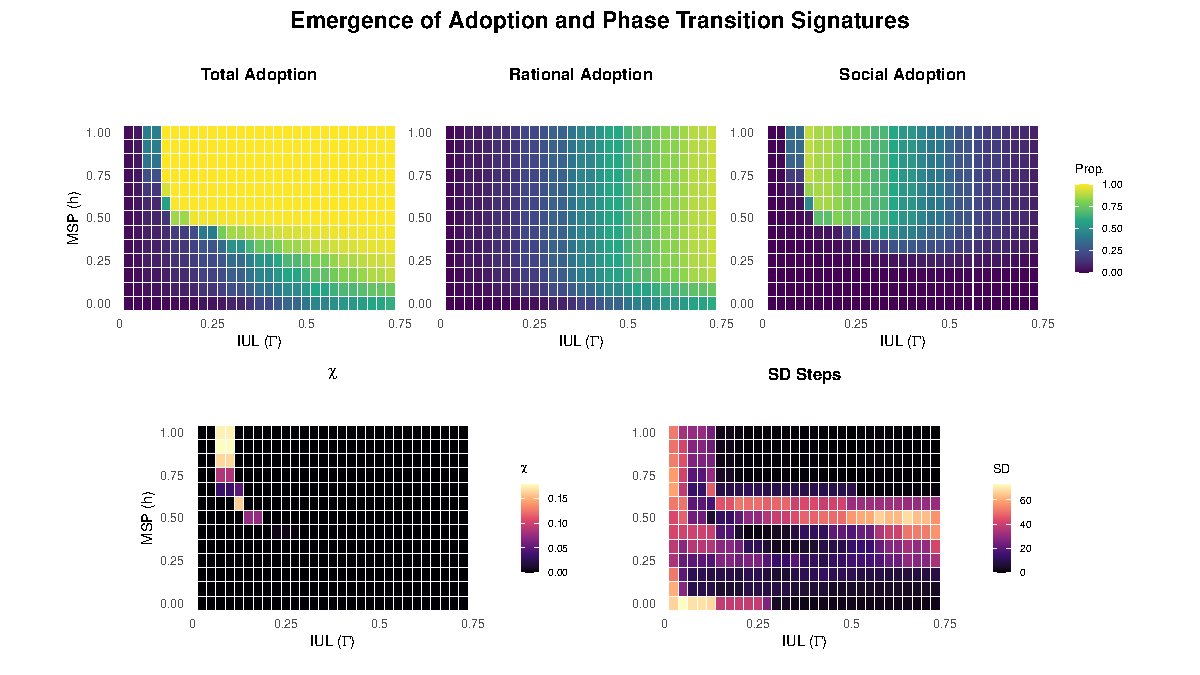
\includegraphics[width=1\textwidth]{../abstract-sn26/figure1_5panels_GSS_ER.pdf}
    \caption{Phase Transition Signatures under generic Degree-Preserving Randomized baselines. Note the complete collapse of variance boundaries and the instantaneous system-wide discontinuity, severing the stable transition regimes found in empirically clustered homophilic topologies.}
    \label{fig:criticality_er}
\end{figure*}

% ==========================================
% SECTION S1: ODD Protocol Summary
% ==========================================
\section{Agent-Based Model: ODD Protocol Summary}

To ensure reproducibility, we outline the primary rules of our social contagion model following the Overview, Design concepts, and Details (ODD) protocol logic.

\paragraph{Initialization (Seeding)} 
Depending on the experimental block, the simulation initializes with either a random node or a strategically pivotal node (e.g., highest Degree, Closeness, Eigenvector). If the selected node requires social reinforcement (threshold count $>1$) to adopt, the algorithm forces adoption on the initiator and iteratively seeds up to the required threshold boundary of the initiator's neighborhood.

\paragraph{Updating (Stochastic Exposure)}
Agent behavior is updated using a stochastic, asynchronous network exposure model via \texttt{netdiffuseR}. At each simulation tick, non-adopters calculate their exposure to adoptions in their local neighborhood. Instead of deterministic synchronous updates---which often trap systems in artificial, oscillating stable states---agents probabilistically transition based on their specific threshold profiles $\tau_i$, which are drawn from $\sim N(\mu, \sigma^2)$ distributions spanning rational and social components.

\paragraph{Stopping Criteria}
The simulation halts under two conditions: (1) an absorbing state is reached wherein no novel adoptions occurred during the current iteration (verified internally by the non-changing diffusion state), or (2) the simulation exceeds a maximum execution limit of $t=200$ steps. Throughout our parameter sweeps, $t=200$ safely encapsulated the full cascade lifetime even at critical phase transitions.

% ==========================================
% SECTION S2
% ==========================================
\newpage
% ==========================================
% SECTION S2
% ==========================================
\newpage
\section{Network Imputation and Topological Validation}

Following McPherson and Smith (2019), we mapped ego-centric data from the General Social Survey (GSS 2004) onto the ATP and GSS macro-samples to construct whole networks ($N=1000$) using Exponential Random Graph Models (ERGMs). 

The reliance on empirical topologies instead of synthetic baselines arises from a fundamental theoretical flaw in typical behavioral modeling. In classic individual-level regression, an implicit assumption is made: \textit{observations are independent conditionally on the covariates} (i.i.d). This assumption is strictly false in sociological contexts because the behavioral outcome $y_i$ of individual $i$ depends on the outcome $y_j$ of individual $j$. Ignoring this relational dependency forces standard estimators to confuse a contextual, topological process with a purely individual effect. McPherson and Smith (2019) addressed this statistical violation by generating an imputed spatial lag $(Wy)$---a matrix of weighted similarities across Blau space---estimating the ``attitudinal climate'' around an individual.

While McPherson's foundational Spatial Autoregressive (SAR) model successfully corrects for homophilic clustering in linear estimators, studying the temporal emergence of collective action via \textit{Social Contagions} demands more than an imputed lag. Agent-Based Models require an explicit, discrete topology---a rigorous definition of exactly ``who is tied to whom.'' 

\subsection{ERGM Generative Simulation and Coefficient Inversion}
To generate these explicit topologies, we utilize Exponential Random Graph Models (ERGMs). The ERGM simulates networks where the probability of a tie dynamically depends on the homophilic distances estimated from the ego-centric data. The coefficients ($\boldsymbol{\beta}_{\text{tot}}$) determining the strength of homophily were derived precisely from the base parameters ($\boldsymbol{\beta}$) and the 2004 temporal shift ($\boldsymbol{\gamma}$) estimated via case-control logistic regression (Smith et al., 2014).

A critical technical adaptation was required to transition between the regression parameterization and the ERGM terms. The original logistic parameters quantified \textit{distance}: a lower (negative) $\beta$ meant that larger socio-demographic disparities reduced tie probability. Conversely, the ERGM algorithm functionally rewards \textit{similarity} for categorical variables through the \texttt{nodematch()} term. Therefore, for categorical variables (Race, Sex, Religion), we formally inverted the sign of the original difference coefficients (e.g., transforming a distance penalty of $-1.352$ into a positive \texttt{nodematch} propensity of $+1.352$). For continuous dimensions (Age, Education), the negative magnitudes were directly preserved via the \texttt{absdiff()} term, penalizing absolute numerical variance.

\subsection{Density Calibration}
To enforce macro-structural realism, the baseline probability of edge formation (the ERGM intercept parameter, \texttt{edges}) underwent iterative computational calibration. The estimation loop iteratively simulated network domains and adjusted the baseline \texttt{edges} penalty until the simulated graph converged on a sparse global target density of exactly $\text{target} = 0.029$. The iterations proceeded until strictly satisfying an absolute density tolerance interval of $\Delta = 0.001$. We generated 100 independent, stable topological realizations to act as our Plausible simulation substrates.

Figures \ref{fig:degree_dist} and \ref{fig:clustering_curves} validate that our generative process yields functional, highly clustered social topologies that preserve right-skewed empirical degree structures—features that synthetic random models systematically fail to emulate jointly.

\begin{figure}[H]
    \centering
    \begin{subfigure}[b]{0.45\textwidth}
        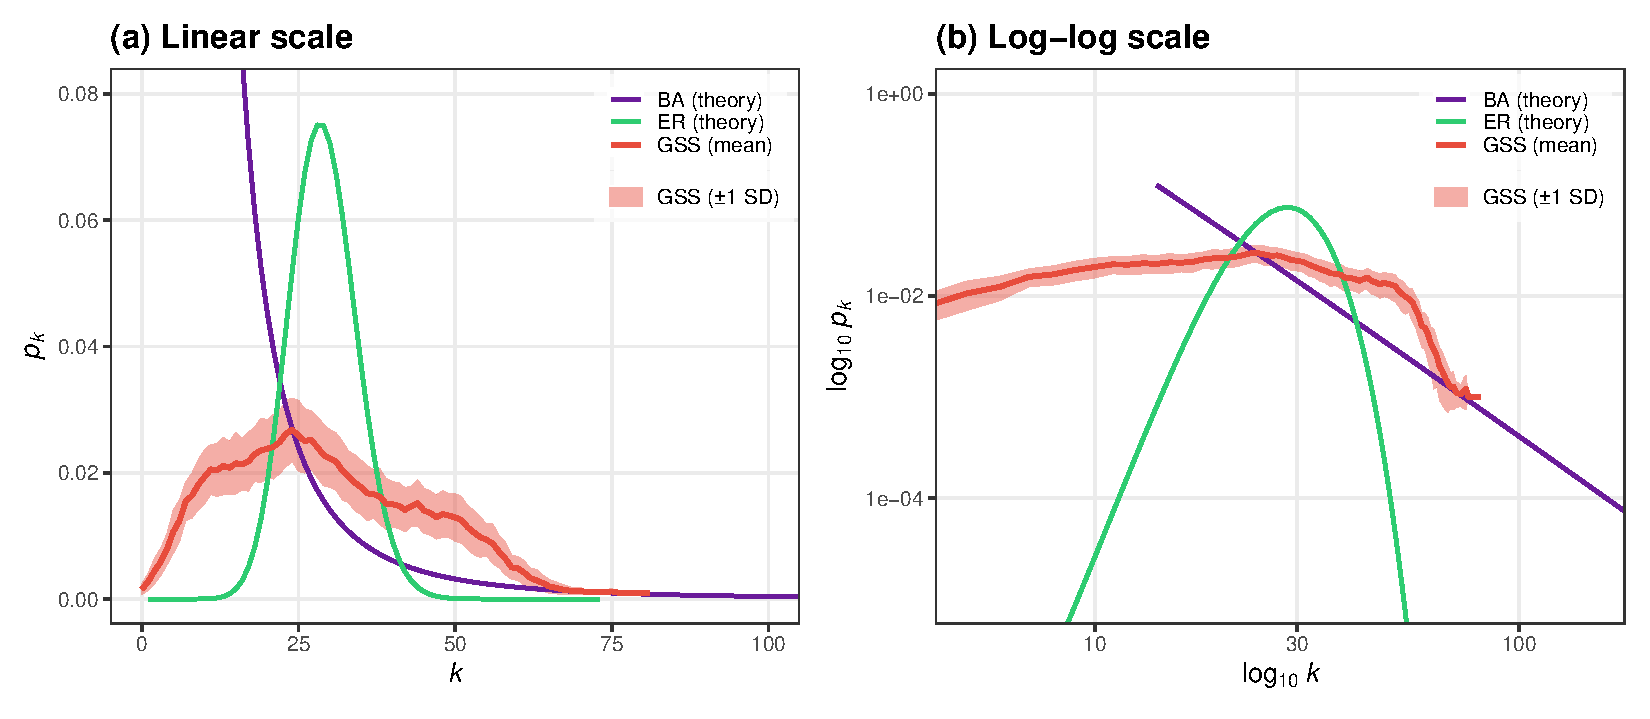
\includegraphics[width=\textwidth]{../../plots/02_GSS_network_ergm_tests/GSS_degree_dist.pdf}
        \caption{GSS respondents.}
    \end{subfigure}
    \hfill
    \begin{subfigure}[b]{0.45\textwidth}
        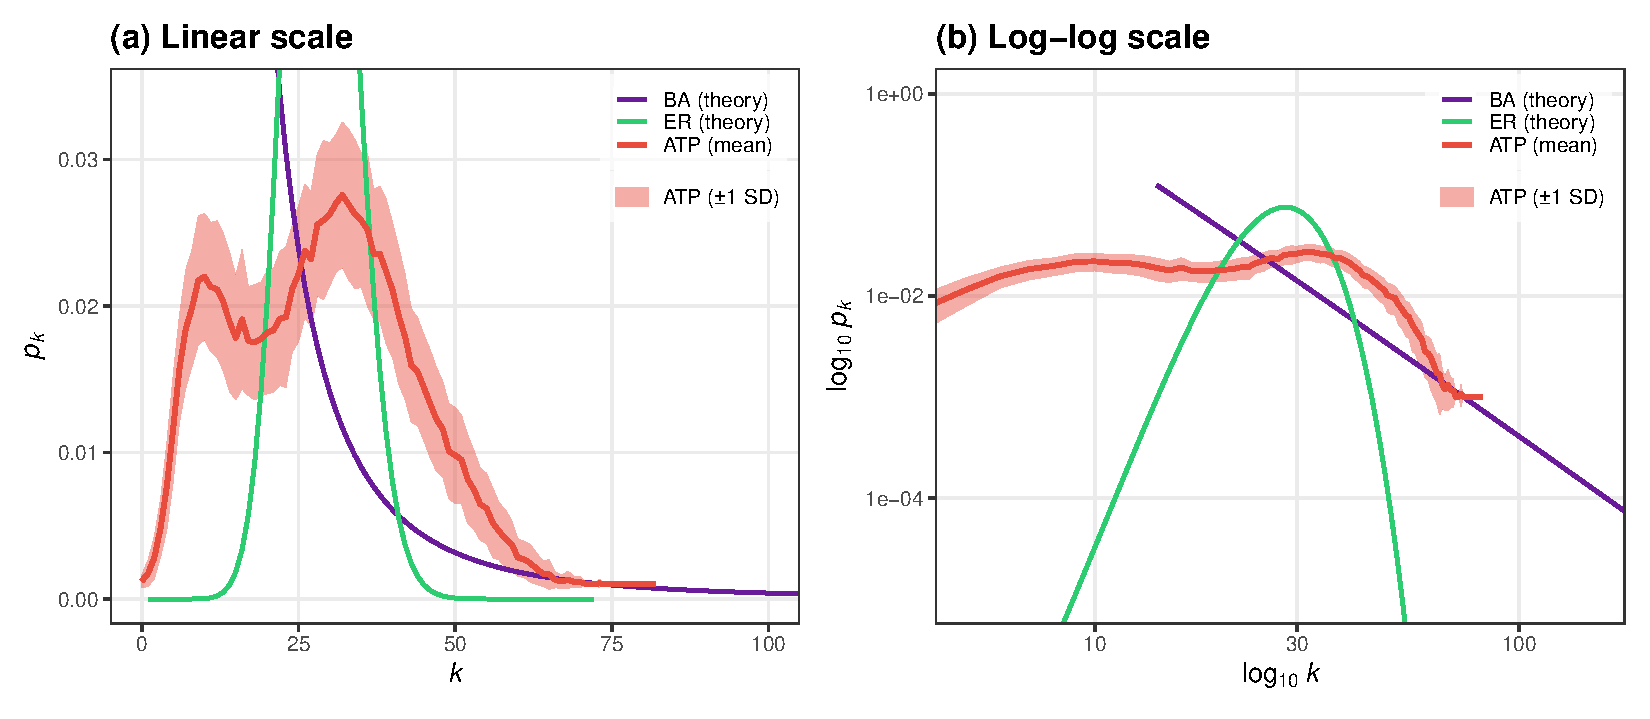
\includegraphics[width=\textwidth]{../../plots/02_ATP_network_ergm_tests/ATP_degree_dist.pdf}
        \caption{ATP respondents.}
    \end{subfigure}
    \caption{Degree distributions of the imputed networks plotted against theoretical models (Degree-Preserving Randomized, Barabási-Albert). The empirical imputations accurately capture real-world right-skewed degree structures.}
    \label{fig:degree_dist}
\end{figure}

\begin{figure}[H]
    \centering
    \begin{subfigure}[b]{0.45\textwidth}
        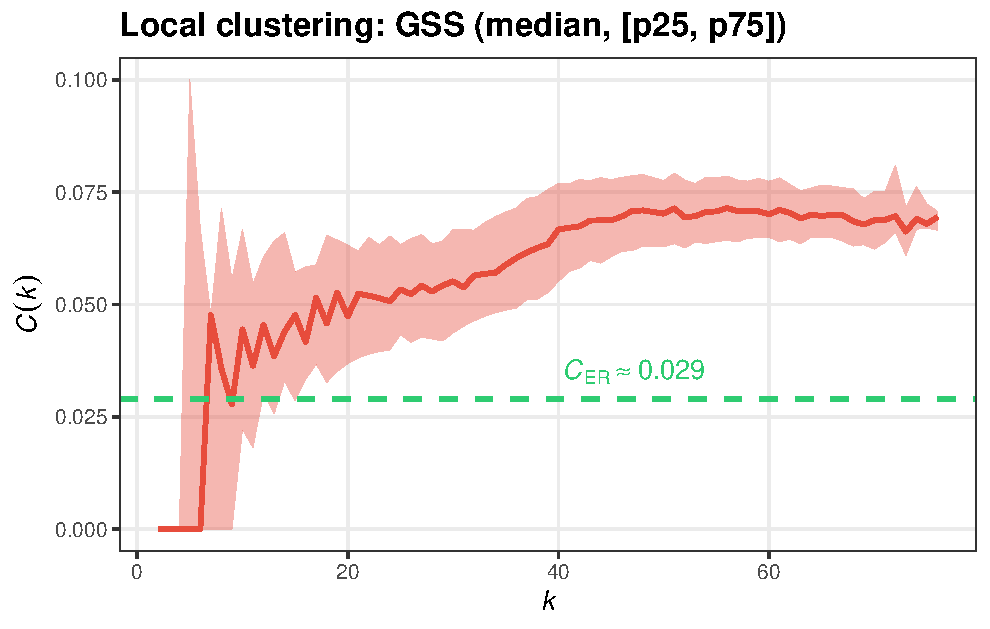
\includegraphics[width=\textwidth]{../../plots/02_GSS_network_ergm_tests/GSS_Ck_vs_k.pdf}
        \caption{Clustering vs. Degree (GSS).}
    \end{subfigure}
    \hfill
    \begin{subfigure}[b]{0.45\textwidth}
        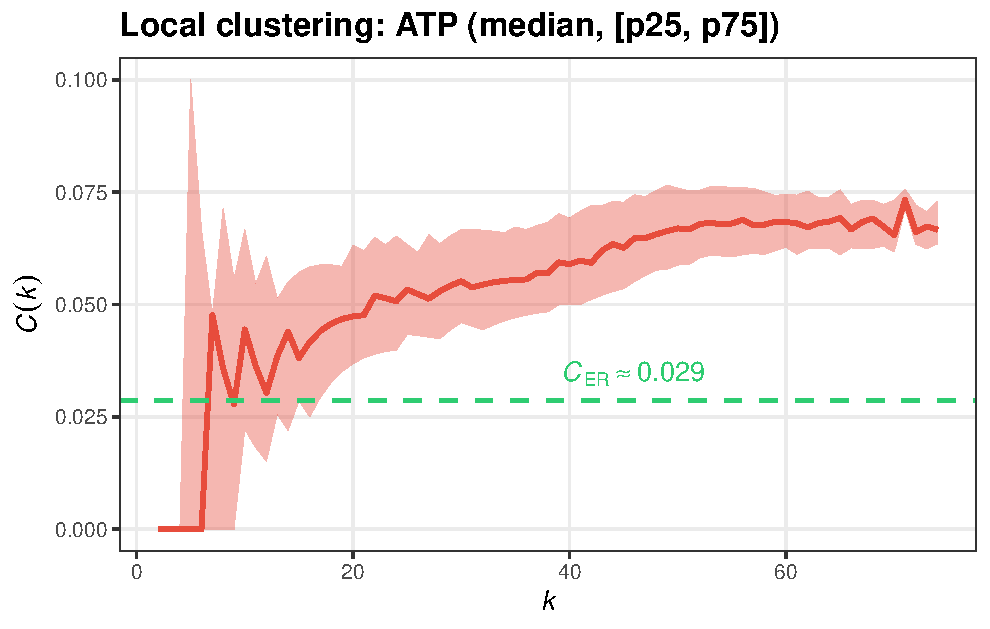
\includegraphics[width=\textwidth]{../../plots/02_ATP_network_ergm_tests/ATP_Ck_vs_k.pdf}
        \caption{Clustering vs. Degree (ATP).}
    \end{subfigure}
    \caption{Local clustering coefficient $C(k)$ as a function of degree $k$. The imputed topologies maintain rich local triad closures characteristic of social structures.}
    \label{fig:clustering_curves}
\end{figure}

% ==========================================
% SECTION S3
% ==========================================
\section{Extended Criticality Analysis: Plausible (GSS) vs. Degree-Preserving Randomized (GSS-DP)}

The mathematical relevance of recovering the critical exponent $\gamma = 1$ in plausible networks in the main text is rooted in Landau's phenomenological theory of phase transitions, contrasted against the unphysical scaling ($\gamma > 3$) observed in degree-preserving randomized topologies. 

\subsection{Mean-Field Derivation}
The free energy density $f(\Phi)$ of the interacting system expanded around the order parameter $\Phi$ is:
\begin{equation}
    f(\Phi) = f_0 + \frac{1}{2}a(T - T_c)\Phi^2 + \frac{1}{4}b\Phi^4 - H\Phi
\end{equation}
Minimizing free energy requires $\frac{\partial f}{\partial \Phi} = 0$. By differentiating the equilibrium condition with respect to an external field $H$, we find the isothermal susceptibility $\chi$:
\begin{equation}
    a(T - T_c)\chi + 3b\Phi^2\chi - 1 = 0 \implies \chi = \frac{1}{a(T - T_c) + 3b\Phi^2}
\end{equation}
As $H \to 0$, $\Phi \to 0$ for $T > T_c$. Thus, susceptibility diverges strictly as $\chi \sim |T - T_c|^{-1}$. Extracting an empirical $\gamma \approx 1$ confirms the system obeys continuous macroscopic scaling.

\subsection{Avalanche Size Spectra and Critical Scaling}
As shown below, empirical GSS (plausible) topologies exhibit scale-free power-law bimodality at criticality, indicative of a second-order transition. The GSS-DP (degree-preserving randomized) graphs exhibit collapsed binary spectra, representing a first-order discontinuity. 
To rigorously trace these transitions, we sweep the simulation domain while fixing the Intrinsic Utility Level (IUL) constant. As the systemic threshold ($MSP$) crosses the empirical boundary $MSP_c$, cascading ``avalanches" (adoption sizes) transition structurally.

\begin{figure}[H]
    \centering
    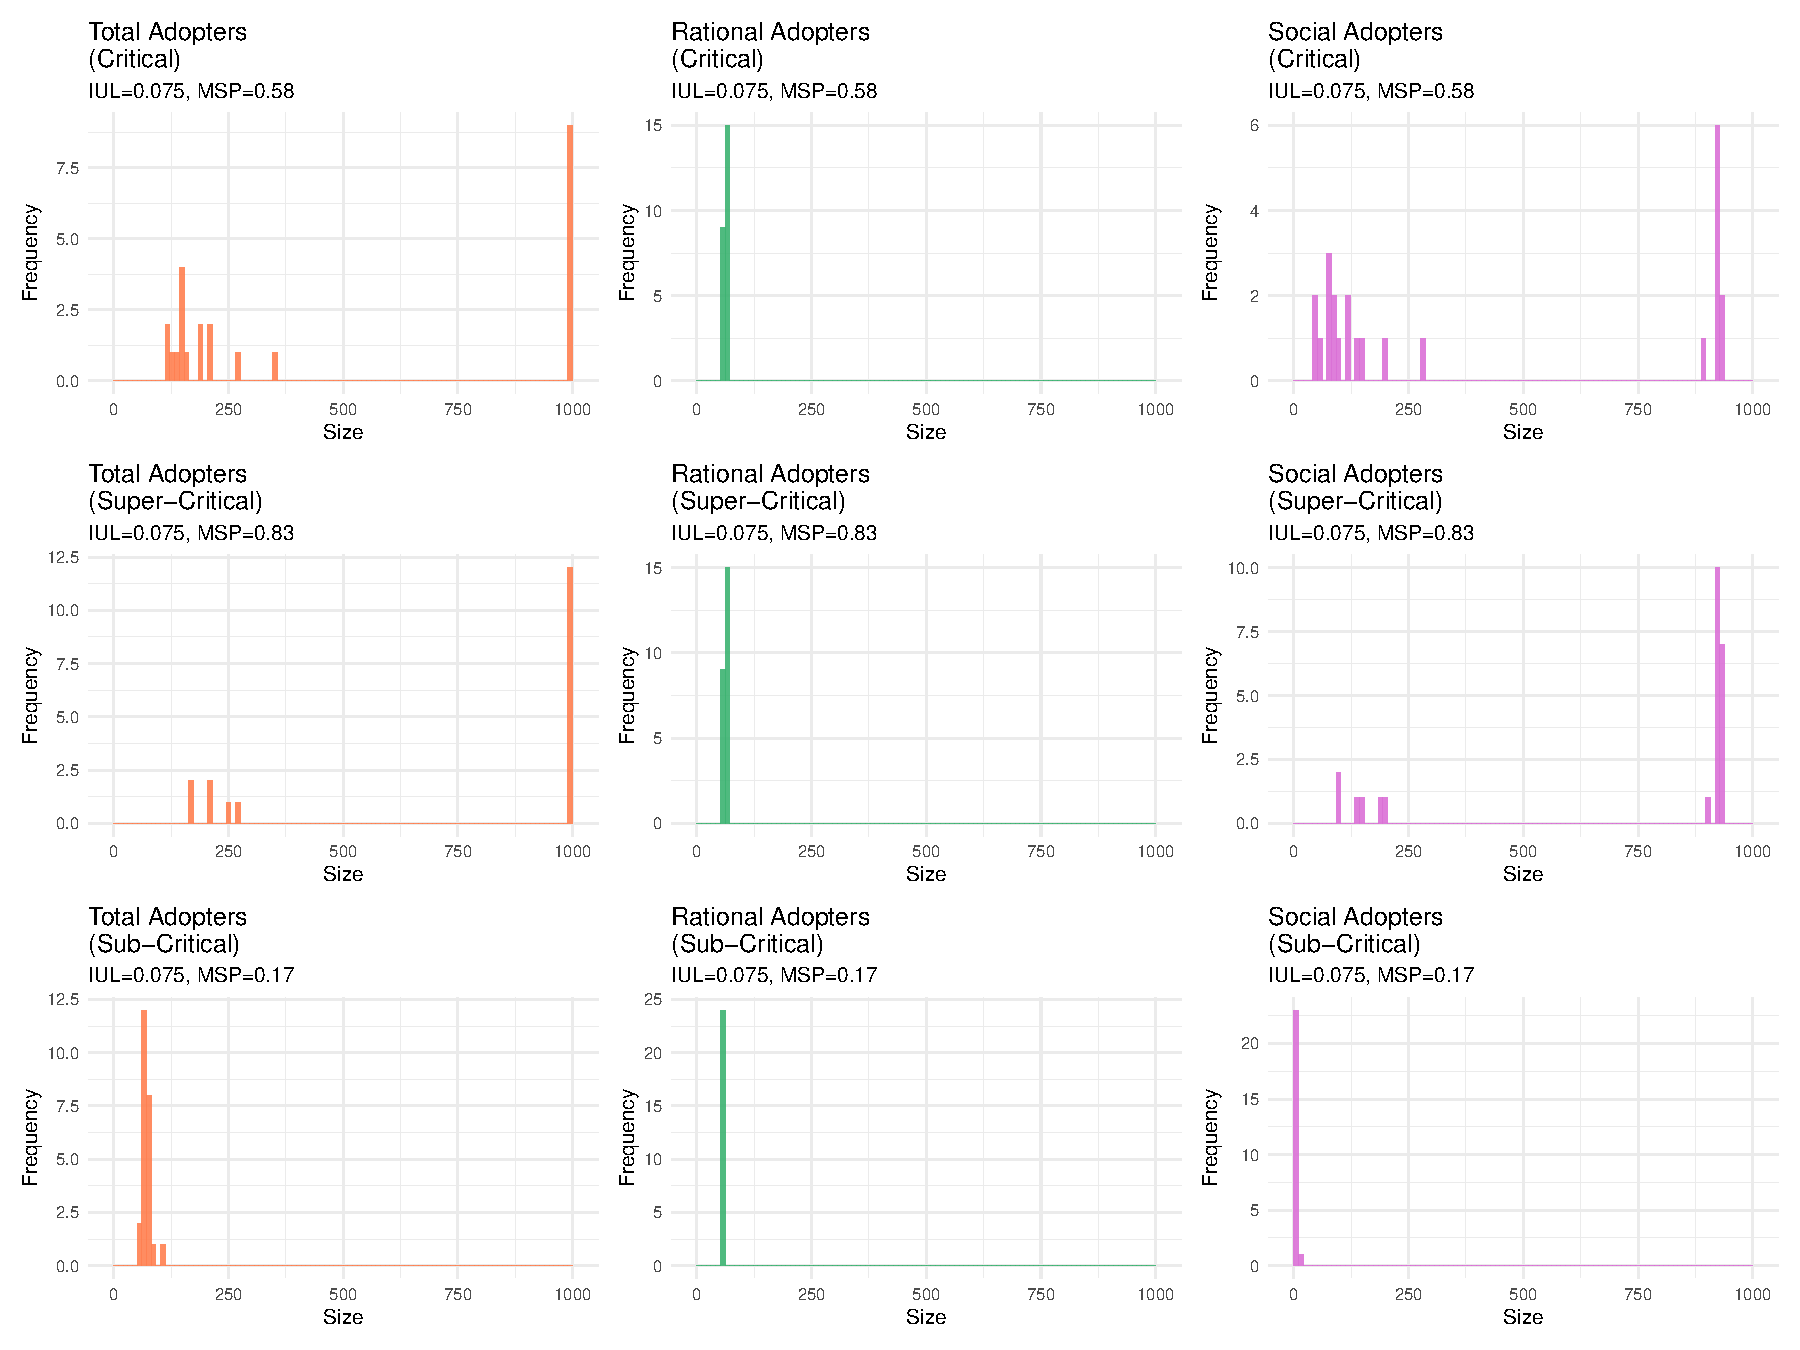
\includegraphics[width=0.8\textwidth]{../../plots/07_phase_transition/GSS/method3_avalanches.pdf}
    \caption{GSS Avalanche Size Spectra: Scale-free power-law bimodality evaluated around the critical variance boundaries $\max(\text{Var}(\Phi))$.}
    \label{fig:spectra_gss}
\end{figure}

\begin{figure}[H]
    \centering
    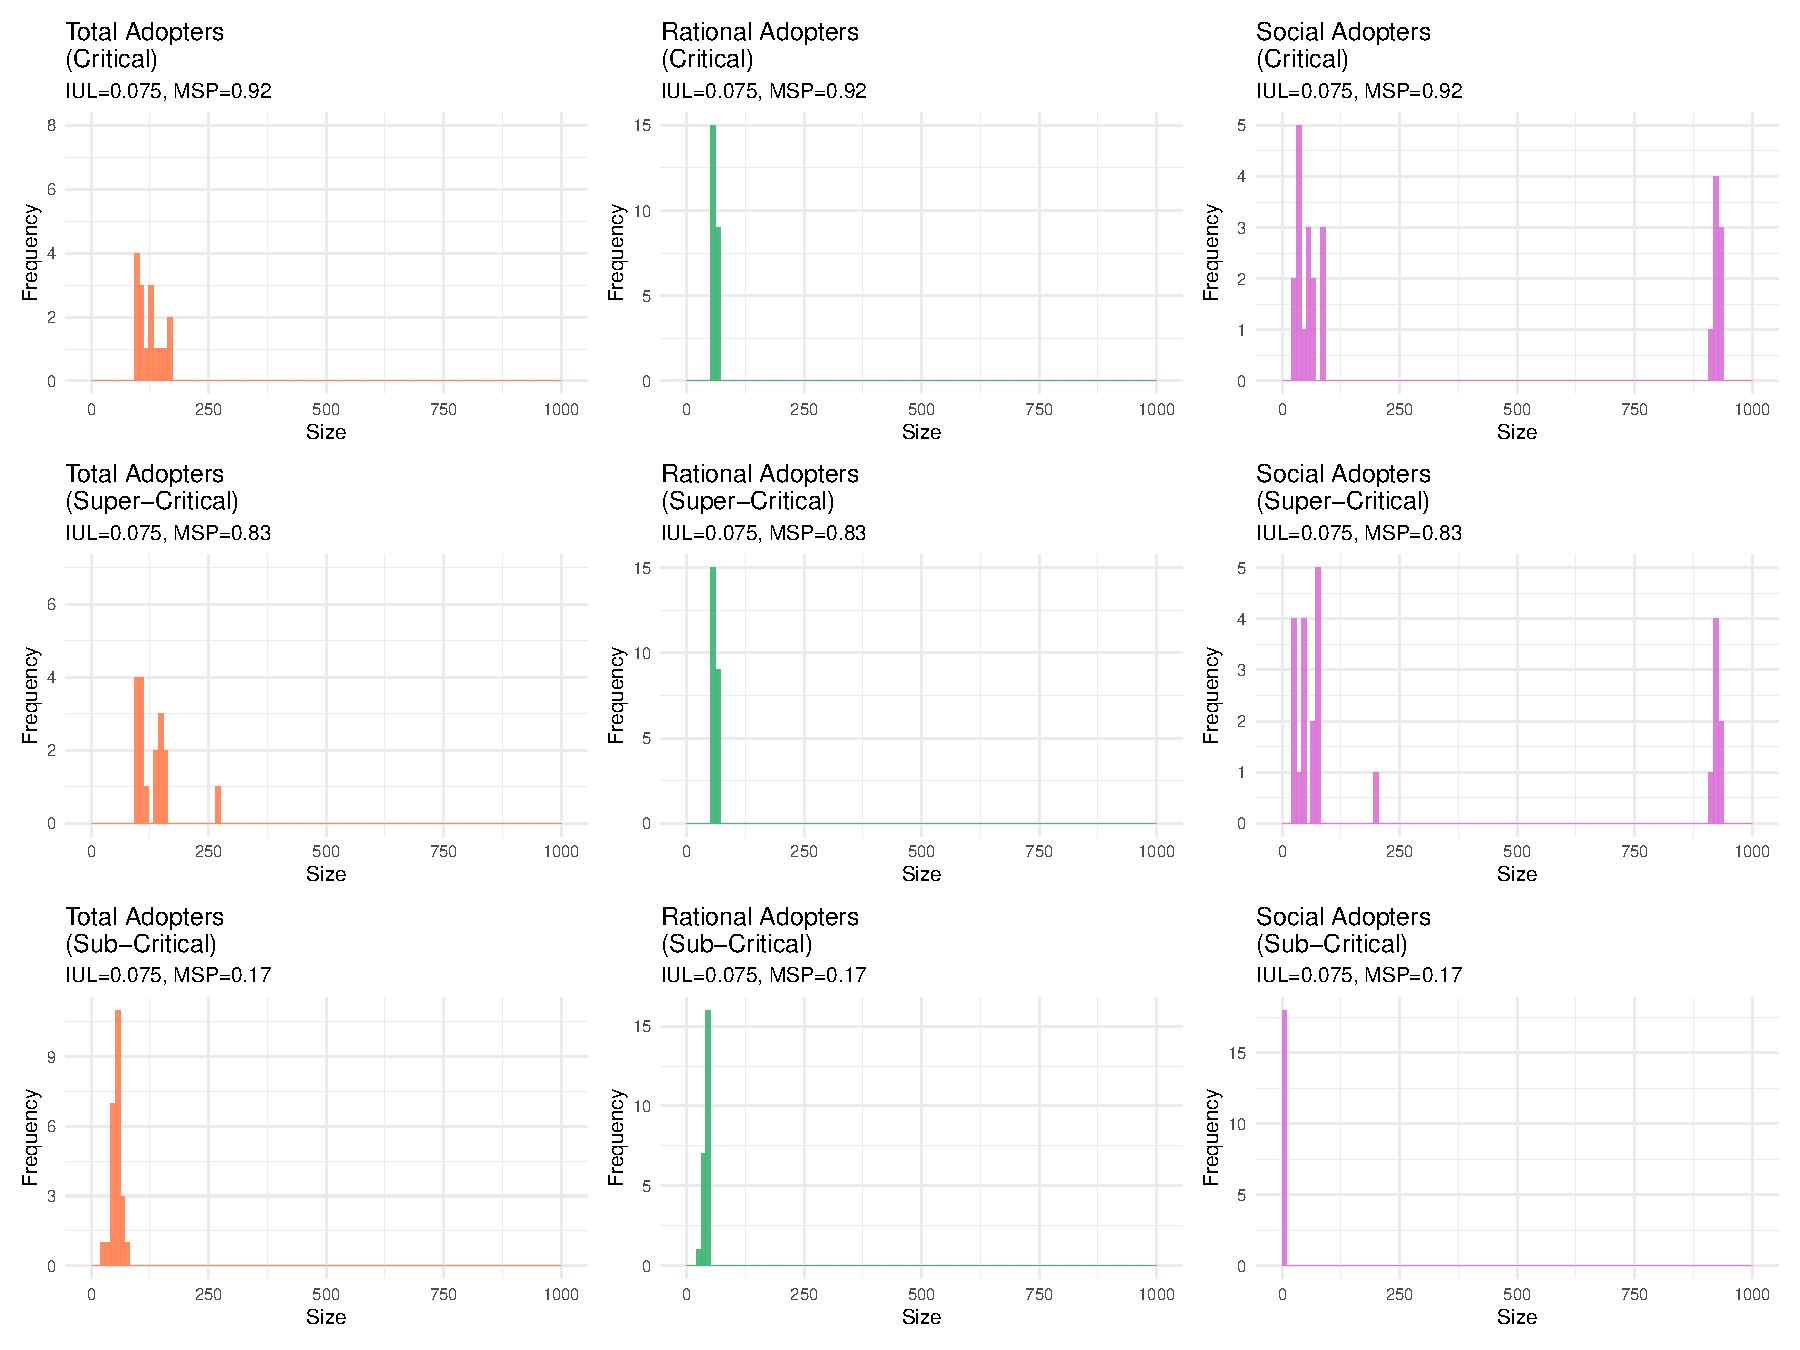
\includegraphics[width=0.8\textwidth]{../../plots/07_phase_transition/GSS_ER/method3_avalanches.pdf}
    \caption{Degree-Preserved Randomization Avalanche Size Spectra: Collapsed binary cascade spectra evaluated around the critical variance boundaries $\max(\text{Var}(\Phi))$.}
    \label{fig:spectra_er}
\end{figure}

\begin{figure}[H]
    \centering
    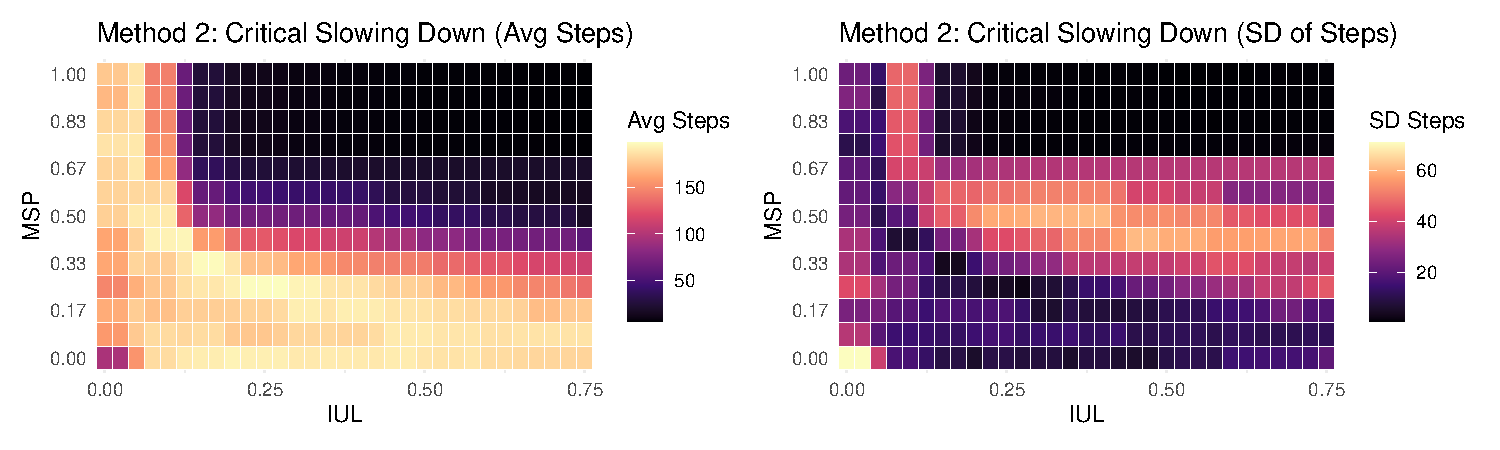
\includegraphics[width=0.8\textwidth]{../../plots/07_phase_transition/GSS/method2_critical_slowing_down.pdf}
    \caption{GSS Critical Slowing Down: Variance of required execution ticks before the structural plateau.}
    \label{fig:csd_gss}
\end{figure}

\begin{figure}[H]
    \centering
    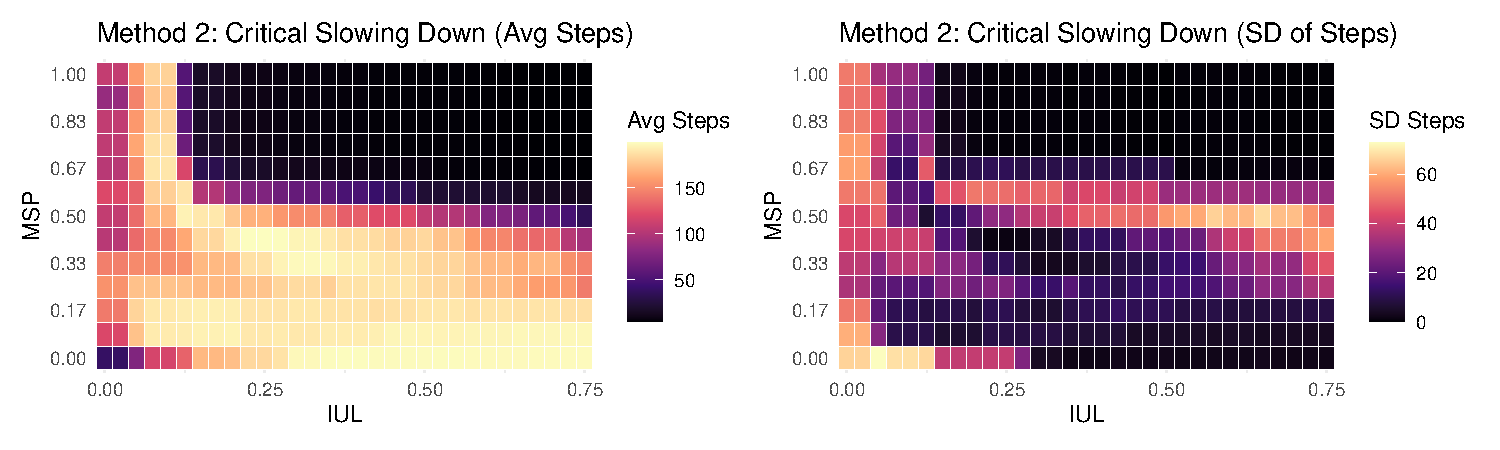
\includegraphics[width=0.8\textwidth]{../../plots/07_phase_transition/GSS_ER/method2_critical_slowing_down.pdf}
    \caption{Degree-Preserved Randomization Critical Slowing Down: Suppressed transition boundaries.}
    \label{fig:csd_er}
\end{figure}

% ==========================================
% SECTION S4
% ==========================================
\section{BAM Regression Model Surfaces}

To ensure the robustness of the structural premium, we explored interacting non-linear terms across multiple dimensions. The following figures visualize the non-linear interaction terms $s(\text{IUL}, \text{MSP})$ estimated by the Big Additive Models (BAMs) across all contagion types (Innovation and Collective Action) for Rational, Social, and Total Adoption.

\begin{figure}[H]
    \centering
    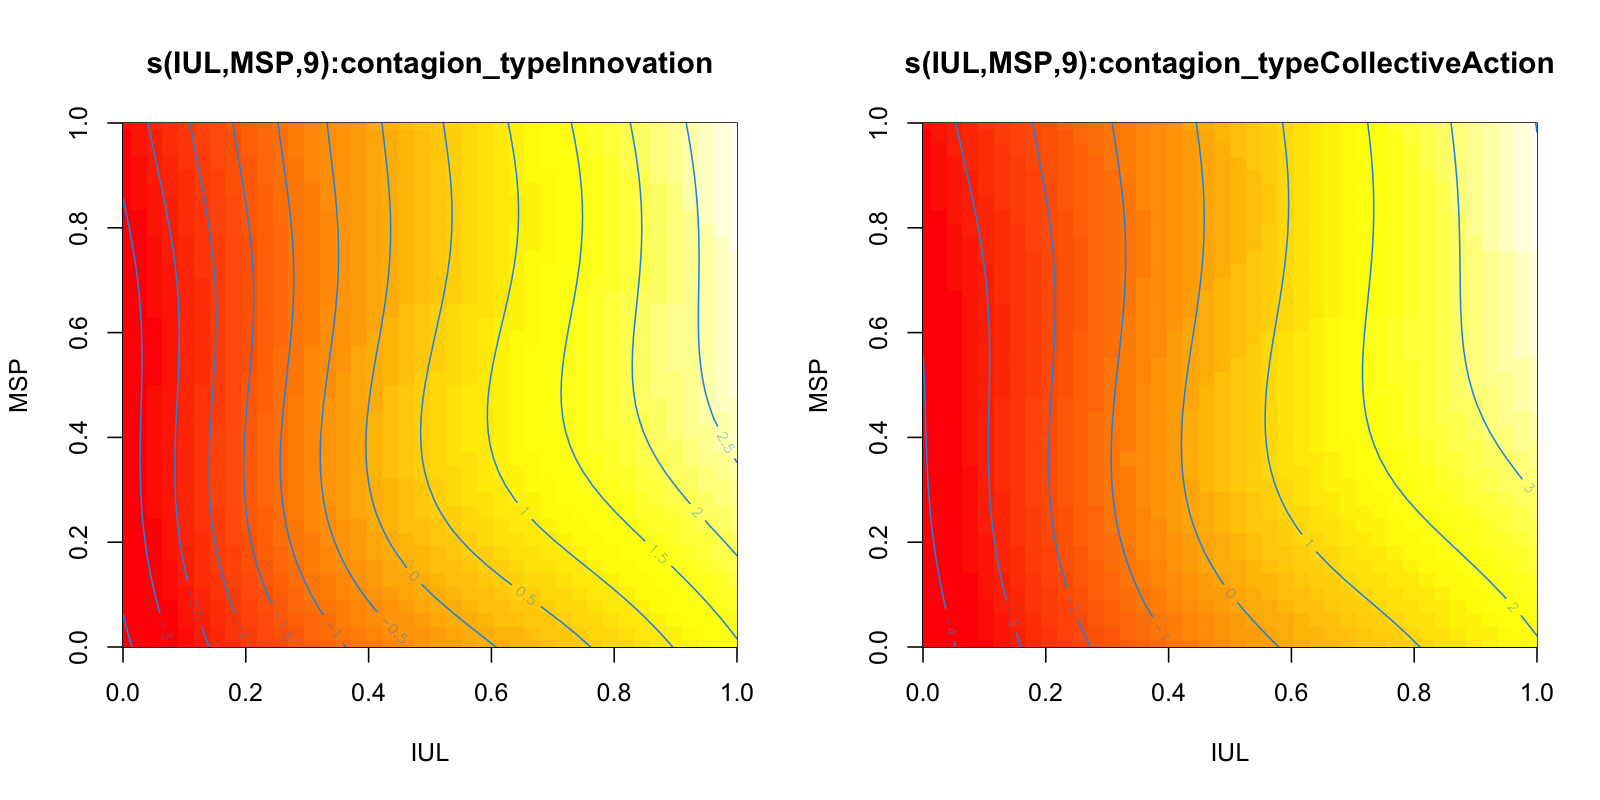
\includegraphics[width=1\linewidth]{../figures/bam_rational_surfaces.png}
    \caption{BAM Smooth Surfaces for Rational Adoption.}
    \label{fig:bam_surfaces_rational}
\end{figure}

\begin{figure}[H]
    \centering
    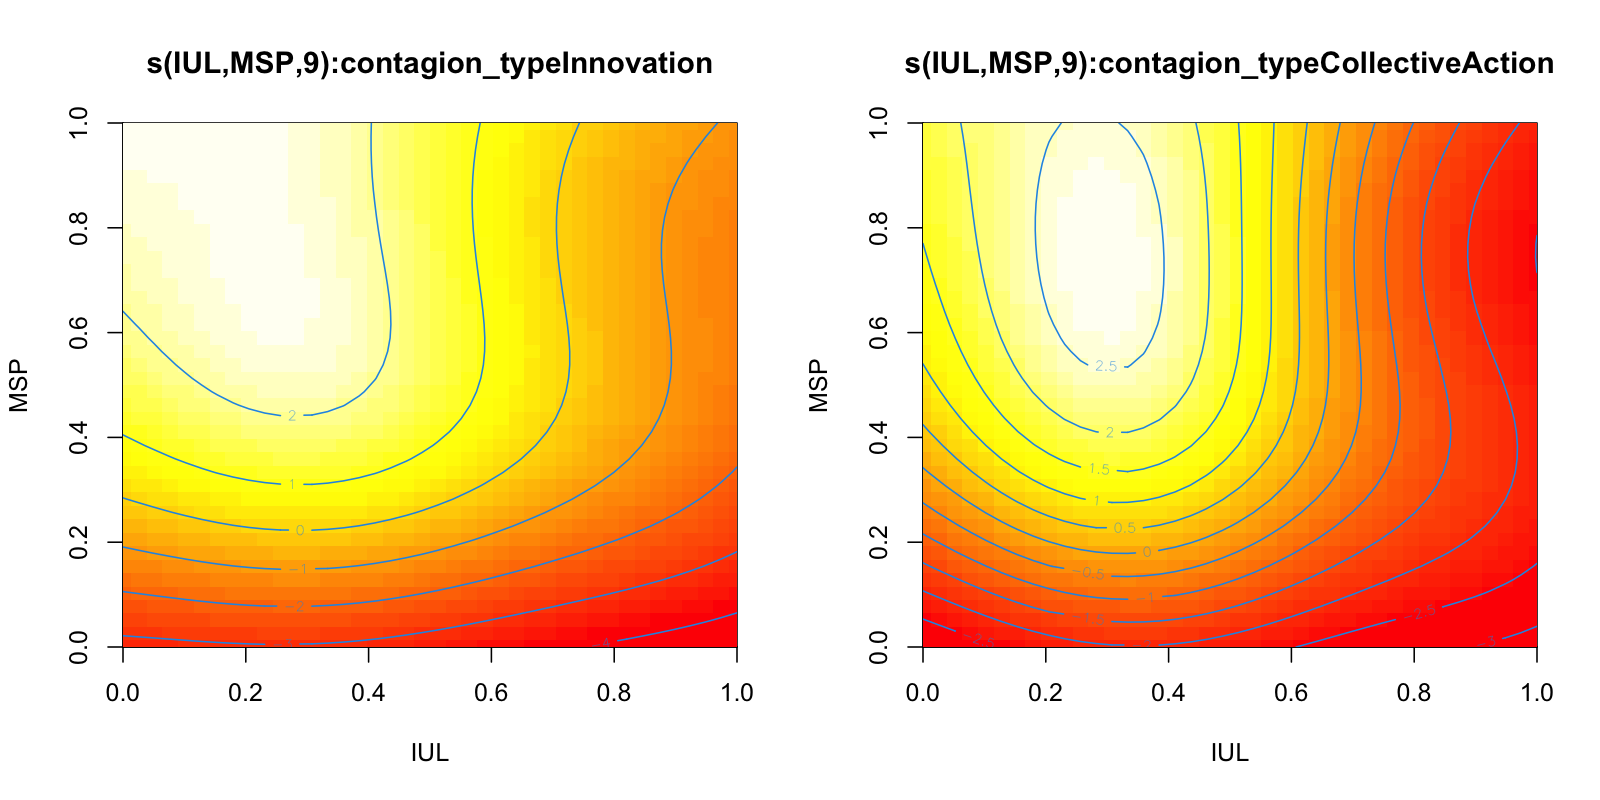
\includegraphics[width=1\linewidth]{../figures/bam_social_surfaces.png}
    \caption{BAM Smooth Surfaces for Social Adoption.}
    \label{fig:bam_surfaces_social}
\end{figure}

\begin{figure}[H]
    \centering
    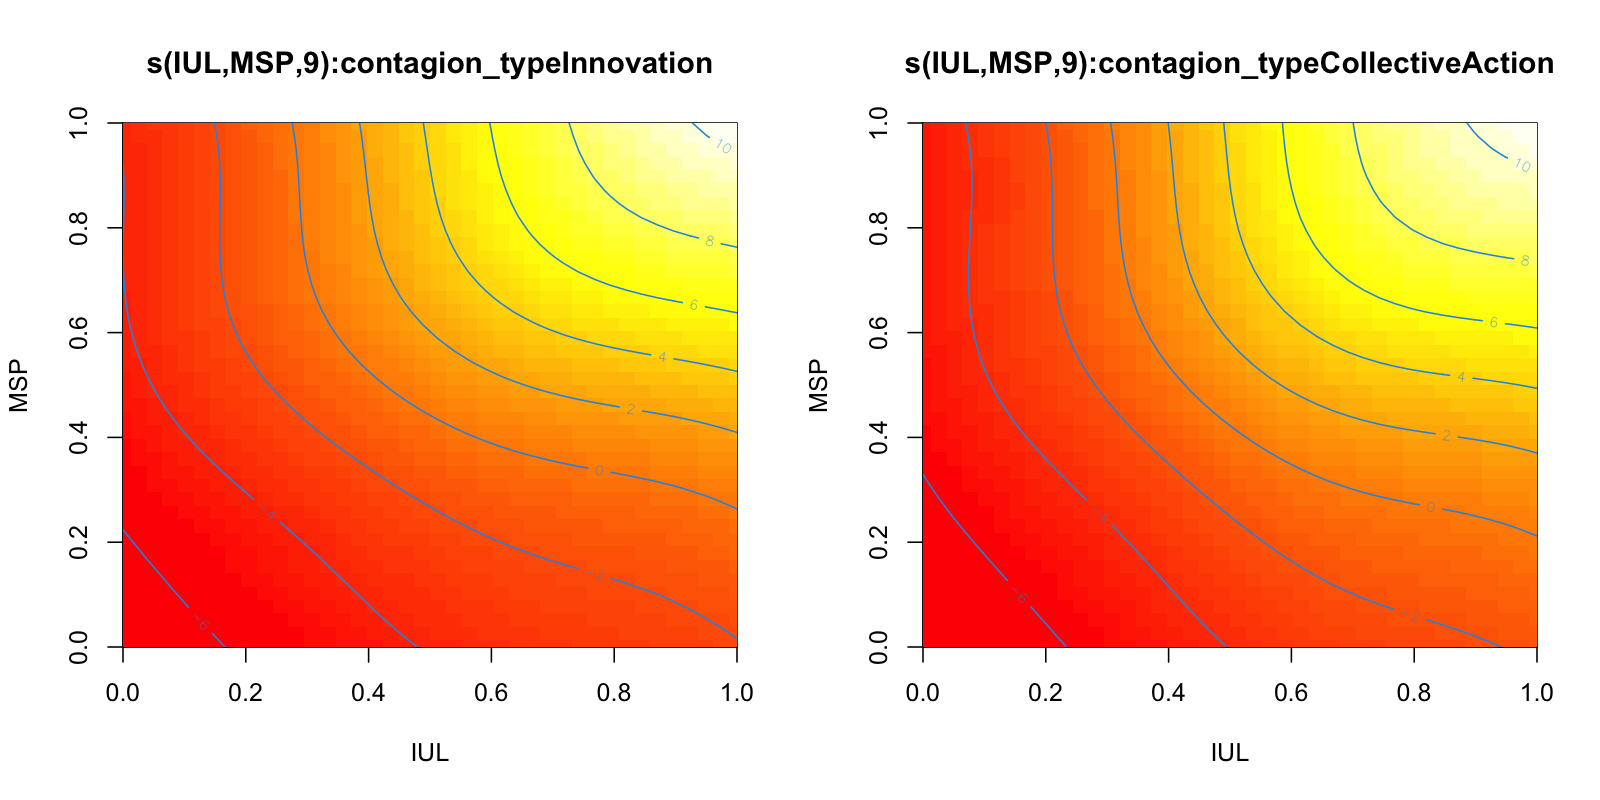
\includegraphics[width=1\linewidth]{../figures/bam_total_surfaces.png}
    \caption{BAM Smooth Surfaces for Total Adoption.}
    \label{fig:bam_surfaces_total}
\end{figure}

\end{document}